%%%%%%%%%%%%%%%%%%%%%%%%%%%%%%%%%%%%%%%%%%%%%%%%%%%%%%%%%%%%%%%%%
% MUW Presentation
% LaTeX Template
% Version 1.0 (27/12/2016)
%
% License:
% CC BY-NC-SA 4.0 (http://creativecommons.org/licenses/by-nc-sa/3.0/)
%
% Created by:
% Nicolas Ballarini, CeMSIIS, Medical University of Vienna
% nicoballarini@gmail.com
% http://statistics.msi.meduniwien.ac.at/
%
% Customized for UAH by:
% David F. Barrero, Departamento de Automática, UAH
%%%%%%%%%%%%%%%%%%%%%%%%%%%%%%%%%%%%%%%%%%%%%%%%%%%%%%%%%%%%%%%%%

\documentclass[10pt,compress]{beamer} % Change 10pt to make fonts of a different size
\mode<presentation>

\usepackage[spanish]{babel}
\usepackage{fontspec}
\usepackage{tikz}
\usepackage{etoolbox}
\usepackage{listings}

\usetheme{UAH}
\usecolortheme{UAH}
\setbeamertemplate{navigation symbols}{} 
\setbeamertemplate{caption}[numbered]

%%%%%%%%%%%%%%%%%%%%%%%%%%%%%%%%%%%%%%%%%%%%%%%%%%%%%%%%%%%%%%%%%
%% Presentation Info
\title[Trabajo Fin de Máster]{Diseño, implementación y evaluación de una estrategia de detección de objetos abandonados en aplicaciones de videovigilancia}
\author{Jesús Mudarra Luján}
\institute{Departamento de Electrónica}
\date{\today}
%%%%%%%%%%%%%%%%%%%%%%%%%%%%%%%%%%%%%%%%%%%%%%%%%%%%%%%%%%%%%%%%%


%%%%%%%%%%%%%%%%%%%%%%%%%%%%%%%%%%%%%%%%%%%%%%%%%%%%%%%%%%%%%%%%%
%% Descomentar para habilitar barra de navegación superior
\setNavigation
%%%%%%%%%%%%%%%%%%%%%%%%%%%%%%%%%%%%%%%%%%%%%%%%%%%%%%%%%%%%%%%%%

%%%%%%%%%%%%%%%%%%%%%%%%%%%%%%%%%%%%%%%%%%%%%%%%%%%%%%%%%%%%%%%%%
%% Configuración de logotipos en portada
%% Opacidad de los logotipos
\newcommand{\opacidad}{1}
%% Descomentar para habilitar logotipo en pié de página de portada
%\renewcommand{\logoUno}{Images/isg.png}
%% Descomentar para habilitar logotipo en pié de página de portada
%\renewcommand{\logoDos}{Images/CCLogo.png}
%% Descomentar para habilitar logotipo en pié de página de portada
%\renewcommand{\logoTres}{Images/ALogo.png}
%% Descomentar para habilitar logotipo en pié de página de portada
%\renewcommand{\logoCuatro}{Images/ELogo.png}
%%%%%%%%%%%%%%%%%%%%%%%%%%%%%%%%%%%%%%%%%%%%%%%%%%%%%%%%%%%%%%%%%

%%%%%%%%%%%%%%%%%%%%%%%%%%%%%%%%%%%%%%%%%%%%%%%%%%%%%%%%%%%%%%%%%
%% FOOTLINE
%% Comment/Uncomment the following blocks to modify the footline
%% content in the body slides. 


%% Option A: Title and institute
\footlineA
%% Option B: Author and institute
%\footlineB
%% Option C: Title, Author and institute
%\footlineC
%%%%%%%%%%%%%%%%%%%%%%%%%%%%%%%%%%%%%%%%%%%%%%%%%%%%%%%%%%%%%%%%%

\begin{document}

%%%%%%%%%%%%%%%%%%%%%%%%%%%%%%%%%%%%%%%%%%%%%%%%%%%%%%%%%%%%%%%%%
% Use this block for a blue title slide with modified footline
{\titlepageBlue
	% Content
    \begin{frame}
        \titlepage
    \end{frame}
}

%%%%%%%%%%%%%%%%%%%%%%%%%%%%%%%%%%%%%%%%%%%%%%%%%%%%%%%%%%%%%%%%%
% Comment/Uncomment these lines for an automatically generated outline.
{\disableNavigation{white}
    \begin{frame}{Índice}
        \tableofcontents
    \end{frame}
}

\addtocounter{framenumber}{-1} %To control the number in which numbering begins

%%%%%%%%%%%%%%%%%%%%%%%%%%%%%%%%%%%%%%%%%%%%%%%%%%%%%%%%%%%%%%%%%
\section{Introducción}
\begin{frame}{Introducción}
\begin{itemize}
  \item Your introduction goes here!
  \item Use \texttt{itemize} to organize your main points.
  \begin{itemize}
  	\item up to 3 text levels with \texttt{itemize}
	\begin{itemize}
  	  	\item Indents increase level by level, font size decreases
		\begin{description}[abc]  % for indentation of length of abc
  			\item[$\bullet$] Should you require more levels, use \texttt{description} instead of \texttt{itemize}.
        	\begin{description}[abc]  % for indentation of length of abc
  				\item[$\bullet$] Note: Please try not to write too much copy onto your slides.
			\end{description}
		\end{description}
	\end{itemize}
  \end{itemize}
  \item Regular \textbf{bold} \textit{italics} \texttt{courier} \textbf{\textit{bold italics}}. 
  \item Description:
    \begin{description}
        \item[Word] This is a nice description
        \item[Another word] This is another nice description
    \end{description}
	\item Enumeration:
	\begin{enumerate}
   		\item This is an \alert{alert}
   		\item This is another \alert{alert}
	\end{enumerate}
  \end{itemize}
\end{frame}


%%%%%%%%%%%%%%%%%%%%%%%%%%%%%%%%%%%%%%%%%%%%%%%%%%%%%%%%%%%%%%%%%
\section{Estudio teórico}
\begin{frame}{Estudio teórico}

\begin{itemize}
  \item You can upload a figure (JPEG, PNG or PDF) using the files menu. 
  \item To include it in your document, use the \texttt{includegraphics} command (see the comment below in the source code).
\end{itemize}

% Commands to include a figure:
\begin{figure}
  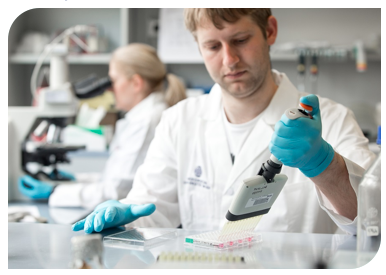
\includegraphics[width=0.5\textwidth]{Images/image.png}
  \caption{\label{fig:your-figure}Caption goes here.}
\end{figure}

\end{frame}


%%%%%%%%%%%%%%%%%%%%%%%%%%%%%%%%%%%%%%%%%%%%%%%%%%%%%%%%%%%%%%%%%
\section{Desarrollo}
\begin{frame}{Sample Chart}
Insert charts as images
\begin{figure}
	\centering
	
\includegraphics[width=0.6\textwidth]{Images/chart.png}
    \caption{Caption}
\end{figure}
\end{frame}

\begin{frame}{Diagrama algoritmo detección de objetos abandonados}

\begin{figure}
	\centering
	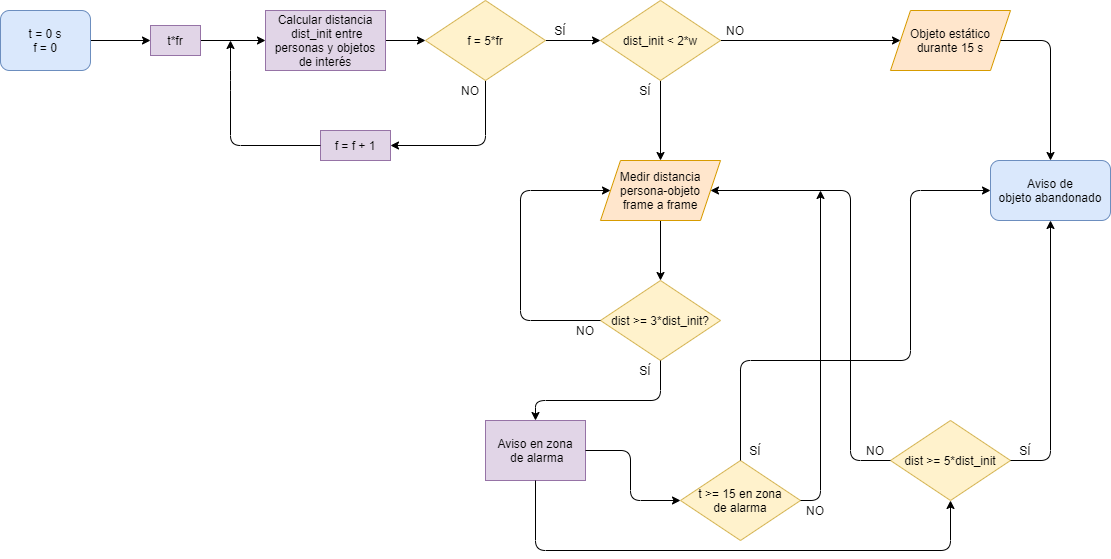
\includegraphics[width=1\textwidth]{Images/desarrollo/abandoned-object-scheme.png}
    \caption{Diagrama algoritmo detección de objetos abandonados}
\end{figure}
\end{frame}


%%%%%%%%%%%%%%%%%%%%%%%%%%%%%%%%%%%%%%%%%%%%%%%%%%%%%%%%%%%%%%%%%
\begin{frame}[t]{Two Columns} %use [t] after \begin{frame} to top alignment
\begin{columns}
  \begin{column}{0.5\textwidth}
    \begin{itemize}
	  \item Left column for content
	  \begin{itemize}
	  	\item Can contain text, charts, pictures, … 
		\end{itemize}
	\end{itemize}
  \end{column}
  \begin{column}{0.5\textwidth}  %%<--- here
    \begin{itemize}
	  \item Right column for content
	  \begin{itemize}
	  	\item Can contain text, charts, pictures, … 
		\end{itemize}
	\end{itemize}
  \end{column}
\end{columns}
\end{frame}


%%%%%%%%%%%%%%%%%%%%%%%%%%%%%%%%%%%%%%%%%%%%%%%%%%%%%%%%%%%%%%%%%
\begin{frame}[t]{Comparison} %use [t] after \begin{frame} to top alignment
\begin{columns}
  \begin{column}{0.5\textwidth}
  	{\large \textcolor{hellblauMUW}{Headline for left column}}
    \begin{itemize}
	  \item Left column for content
	  \begin{itemize}
	  	\item Can contain text, charts, pictures, … 
		\end{itemize}
	\end{itemize}
  \end{column}
  \begin{column}{0.5\textwidth}  %%<--- here
  {\large \textcolor{hellblauMUW}{Headline for right column}}
    \begin{itemize}
	  \item Right column for content
	  \begin{itemize}
	  	\item Can contain text, charts, pictures, … 
		\end{itemize}
	\end{itemize}
  \end{column}
\end{columns}
\end{frame}


%%%%%%%%%%%%%%%%%%%%%%%%%%%%%%%%%%%%%%%%%%%%%%%%%%%%%%%%%%%%%%%%%
\begin{frame}{Blocks}

\begin{block}{Block}
Some examples of commonly used commands and features are included, to help you get started.
\end{block}

\begin{exampleblock}{Example Block}
Some examples of commonly used commands and features are included, to help you get started.
\end{exampleblock}

\begin{alertblock}{Alert Block}
Some examples of commonly used commands and features are included, to help you get started.
\end{alertblock}

\end{frame}

%%%%%%%%%%%%%%%%%%%%%%%%%%%%%%%%%%%%%%%%%%%%%%%%%%%%%%%%%%%%%%%%%
\section{Resultados}
\subsection{Tables}

\begin{frame}{Tables}

\begin{table}
\centering
\begin{tabular}{l|r}
Item & Quantity \\\hline
Widgets & 42 \\
Gadgets & 13
\end{tabular}
\caption{\label{tab:widgets}An example table.}
\end{table}

\end{frame}

%%%%%%%%%%%%%%%%%%%%%%%%%%%%%%%%%%%%%%%%%%%%%%%%%%%%%%%%%%%%%%%%%
\subsection{Source code}

\begin{frame}{Source code}
    \begin{columns}
 	   \column{.50\textwidth}
	        \begin{block}{Python}
	        \vspace{-0.2cm}
		        \lstinputlisting{code/hello.py}
            \end{block}
 	   \column{.50\textwidth}
		    \lstinputlisting[language=C]{code/hello.c}
    \end{columns}
\end{frame}

%%%%%%%%%%%%%%%%%%%%%%%%%%%%%%%%%%%%%%%%%%%%%%%%%%%%%%%%%%%%%%%%%
\subsection{Mathematics}

\begin{frame}{Readable Mathematics}

Let $X_1, X_2, \ldots, X_n$ be a sequence of independent and identically distributed random variables with $\text{E}[X_i] = \mu$ and $\text{Var}[X_i] = \sigma^2 < \infty$, and let
$$S_n = \frac{X_1 + X_2 + \cdots + X_n}{n}
      = \frac{1}{n}\sum_{i}^{n} X_i$$
denote their mean. Then as $n$ approaches infinity, the random variables $\sqrt{n}(S_n - \mu)$ converge in distribution to a normal $\mathcal{N}(0, \sigma^2)$.

\end{frame}


%%%%%%%%%%%%%%%%%%%%%%%%%%%%%%%%%%%%%%%%%%%%%%%%%%%%%%%%%%%%%%%%%
\section{Conclusiones}
\begin{frame}{Conclusiones}

\begin{itemize}
  \item You can upload a figure (JPEG, PNG or PDF) using the files menu. 
  \item To include it in your document, use the \texttt{includegraphics} command (see the comment below in the source code).
\end{itemize}

% Commands to include a figure:
\begin{figure}
  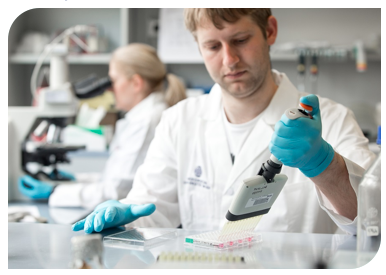
\includegraphics[width=0.5\textwidth]{Images/image.png}
  \caption{\label{fig:your-figure2}Caption goes here2.}
\end{figure}

\end{frame}


%%%%%%%%%%%%%%%%%%%%%%%%%%%%%%%%%%%%%%%%%%%%%%%%%%%%%%%%%%%%%%%%%
\section{Líneas futuras}
\begin{frame}{Líneas futuras}

\begin{itemize}
  \item You can upload a figure (JPEG, PNG or PDF) using the files menu. 
  \item To include it in your document, use the \texttt{includegraphics} command (see the comment below in the source code).
\end{itemize}

% Commands to include a figure:
\begin{figure}
  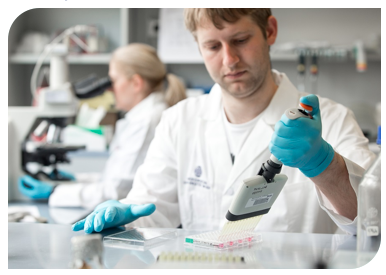
\includegraphics[width=0.5\textwidth]{Images/image.png}
  \caption{\label{fig:your-figure3}Caption goes here3.}
\end{figure}

\end{frame}


%%%%%%%%%%%%%%%%%%%%%%%%%%%%%%%%%%%%%%%%%%%%%%%%%%%%%%%%%%%%%%%%%
\section*{¿Preguntas?}
{
\sectionheaderWhite 

\begin{frame}{¡Muchas gracias por su atención!}{¿Preguntas?}
\end{frame}

}

\end{document}